\chapter{Background and Related Work}

\section{Terminology \ar Glossary?}

\paragraph{Planar image}
\paragraph{360\degree image}
\paragraph{Interpolation vs Synthesis} In the context of this thesis, the two terms are very similar. Interpolation is used as a type of synthesis where two images are weighted by a certain amount and added together \ldots ?
\paragraph{Viewpoint, capture, camera} input viewpoint, output viewpoint
Capture/Viewpoint is the term used here to signify the location and image data of a 360\degree photograph taken at a certain position in the scene
capture is more for when the images are actually recorded
viewpoint is more for during processing
\paragraph{UV coordinates}
image-based rendering vs pixel-based rendering

%\section{Fundamentals of 360\degree Images}
\section{Fundamentals}

\subsection{360\degree Images}
Capturing an image with a 360\degree camera can be regarded mathematically as a series of projections. The sensors of a 360\degree camera can be simplified as a unit sphere covered in light receptors, where the number of light receptors corresponds to the resolution of the camera. This means that the complete surroundings are projected onto this sphere by way of incoming light rays (see Figure~\ref{lightrays}). The limited number of sensors acts as a discretizer and captures a specific color value for each resolution point (pixel). At this point, the data is in \emph{world coordinates}, meaning that each pixel value corresponds to a point on the surface of the unit sphere. 
\missingfigure{incoming light rays on unit sphere, maybe with uv indices \label{lightrays}}

As the majority of viewing devices is planar (e.g. computer or smartphone screens), the image data needs to be projected to a flat surface in order to be viewed on a flat screen. This problem is well-known in cartography, and several different types of projections exist, which transform the data from world coordinates to \emph{image coordinates}.

\subsubsection{Projections for Planar Viewing \label{projections} \cite{hdrbook}}
The most common projections for 360\degree images are the \emph{ideal mirrored sphere}, the \emph{angular map},  \emph{equirectangular}, also known as \emph{latitude-longitude} (\emph{latlong}) and the \emph{cube map} \cite{hdrbook}.

\paragraph{Cube Map}
The cube map is a mapping that splits the data into six separate square views, one in each direction (top, front, left, right, back, bottom). This is the equivalent of capturing the surroundings with six different cameras with a field of view of 90\degree each and stitching the resulting images together in a shape that can be ``folded'' into a cube (see Figure~\ref{fig:cubemap-intro}), which also gives this mapping its name.
Due to the projection of each side to a plane, there is some distortion towards the edges of each face, though this distortion is limited, which is a significant advantage compared to other mappings. The disadvantage is that there are many seams and there tend to be directional discontinuities at these seams. This type of mapping is often used to simulate complex environments in 3D scenes (e.g. for game or animation graphics), as it is easy to use and reduces render time significantly compared to a 3D model of the same environment.
\cite{hdrbook}

\paragraph{Ideal Mirrored Sphere}
The ideal mirrored sphere is a mapping to a circle within a square. It represents how the surroundings would be reflected by a perfect mirrored sphere, given the size of the sphere was considerably smaller than the distance to the surroundings. This mapping, like all the mappings presented here, shows the complete surroundings, albeit very distorted toward the edges. Figure~\ref{spheremaps}~(b) shows where each direction is mapped and the extent of the distortion. It is clear that the farther away from the ``front'' area, the more distorted the mirrored sphere mapping is. The ideal mirrored sphere mapping can be used for calculating average illumination color for high dynamic range calculations, however, the type of distortion at the edges can cause problems with sampling, which is why the angular map mapping tends to be preferred.
\cite{hdrbook}

\paragraph{Angular Map}
At first sight, the angular map seems very similar to the ideal mirrored sphere. It also maps to a circle within a square, however it samples the input in such a way that the back of the image is allotted more space and is less distorted than the mirrored sphere (see Figure~\ref{fig:angular-intro}). This mapping is also used for high dynamic range calculations.

\paragraph{Equirectangular}
The equirectangular, or latitude-longitude mapping is a common type of mapping in cartography. The data is mapped to a rectangular image space, in which the width is twice the height. The azimuth (around the circumference) of the world coordinates is mapped to the map's horizontal coordinate and the elevation to the vertical coordinate. This representation suffers from the same problem as is known from cartography: The distortion increases significantly towards the poles, as can be seen in Figure~\ref{fig:latlong-intro}. Otherwise, this mapping is convenient as it has very few seams. It is used as a storage format for 360\degree images.

\begin{figure}
\centering
    \begin{subfigure}[b]{0.5\textwidth}            
            \centering
            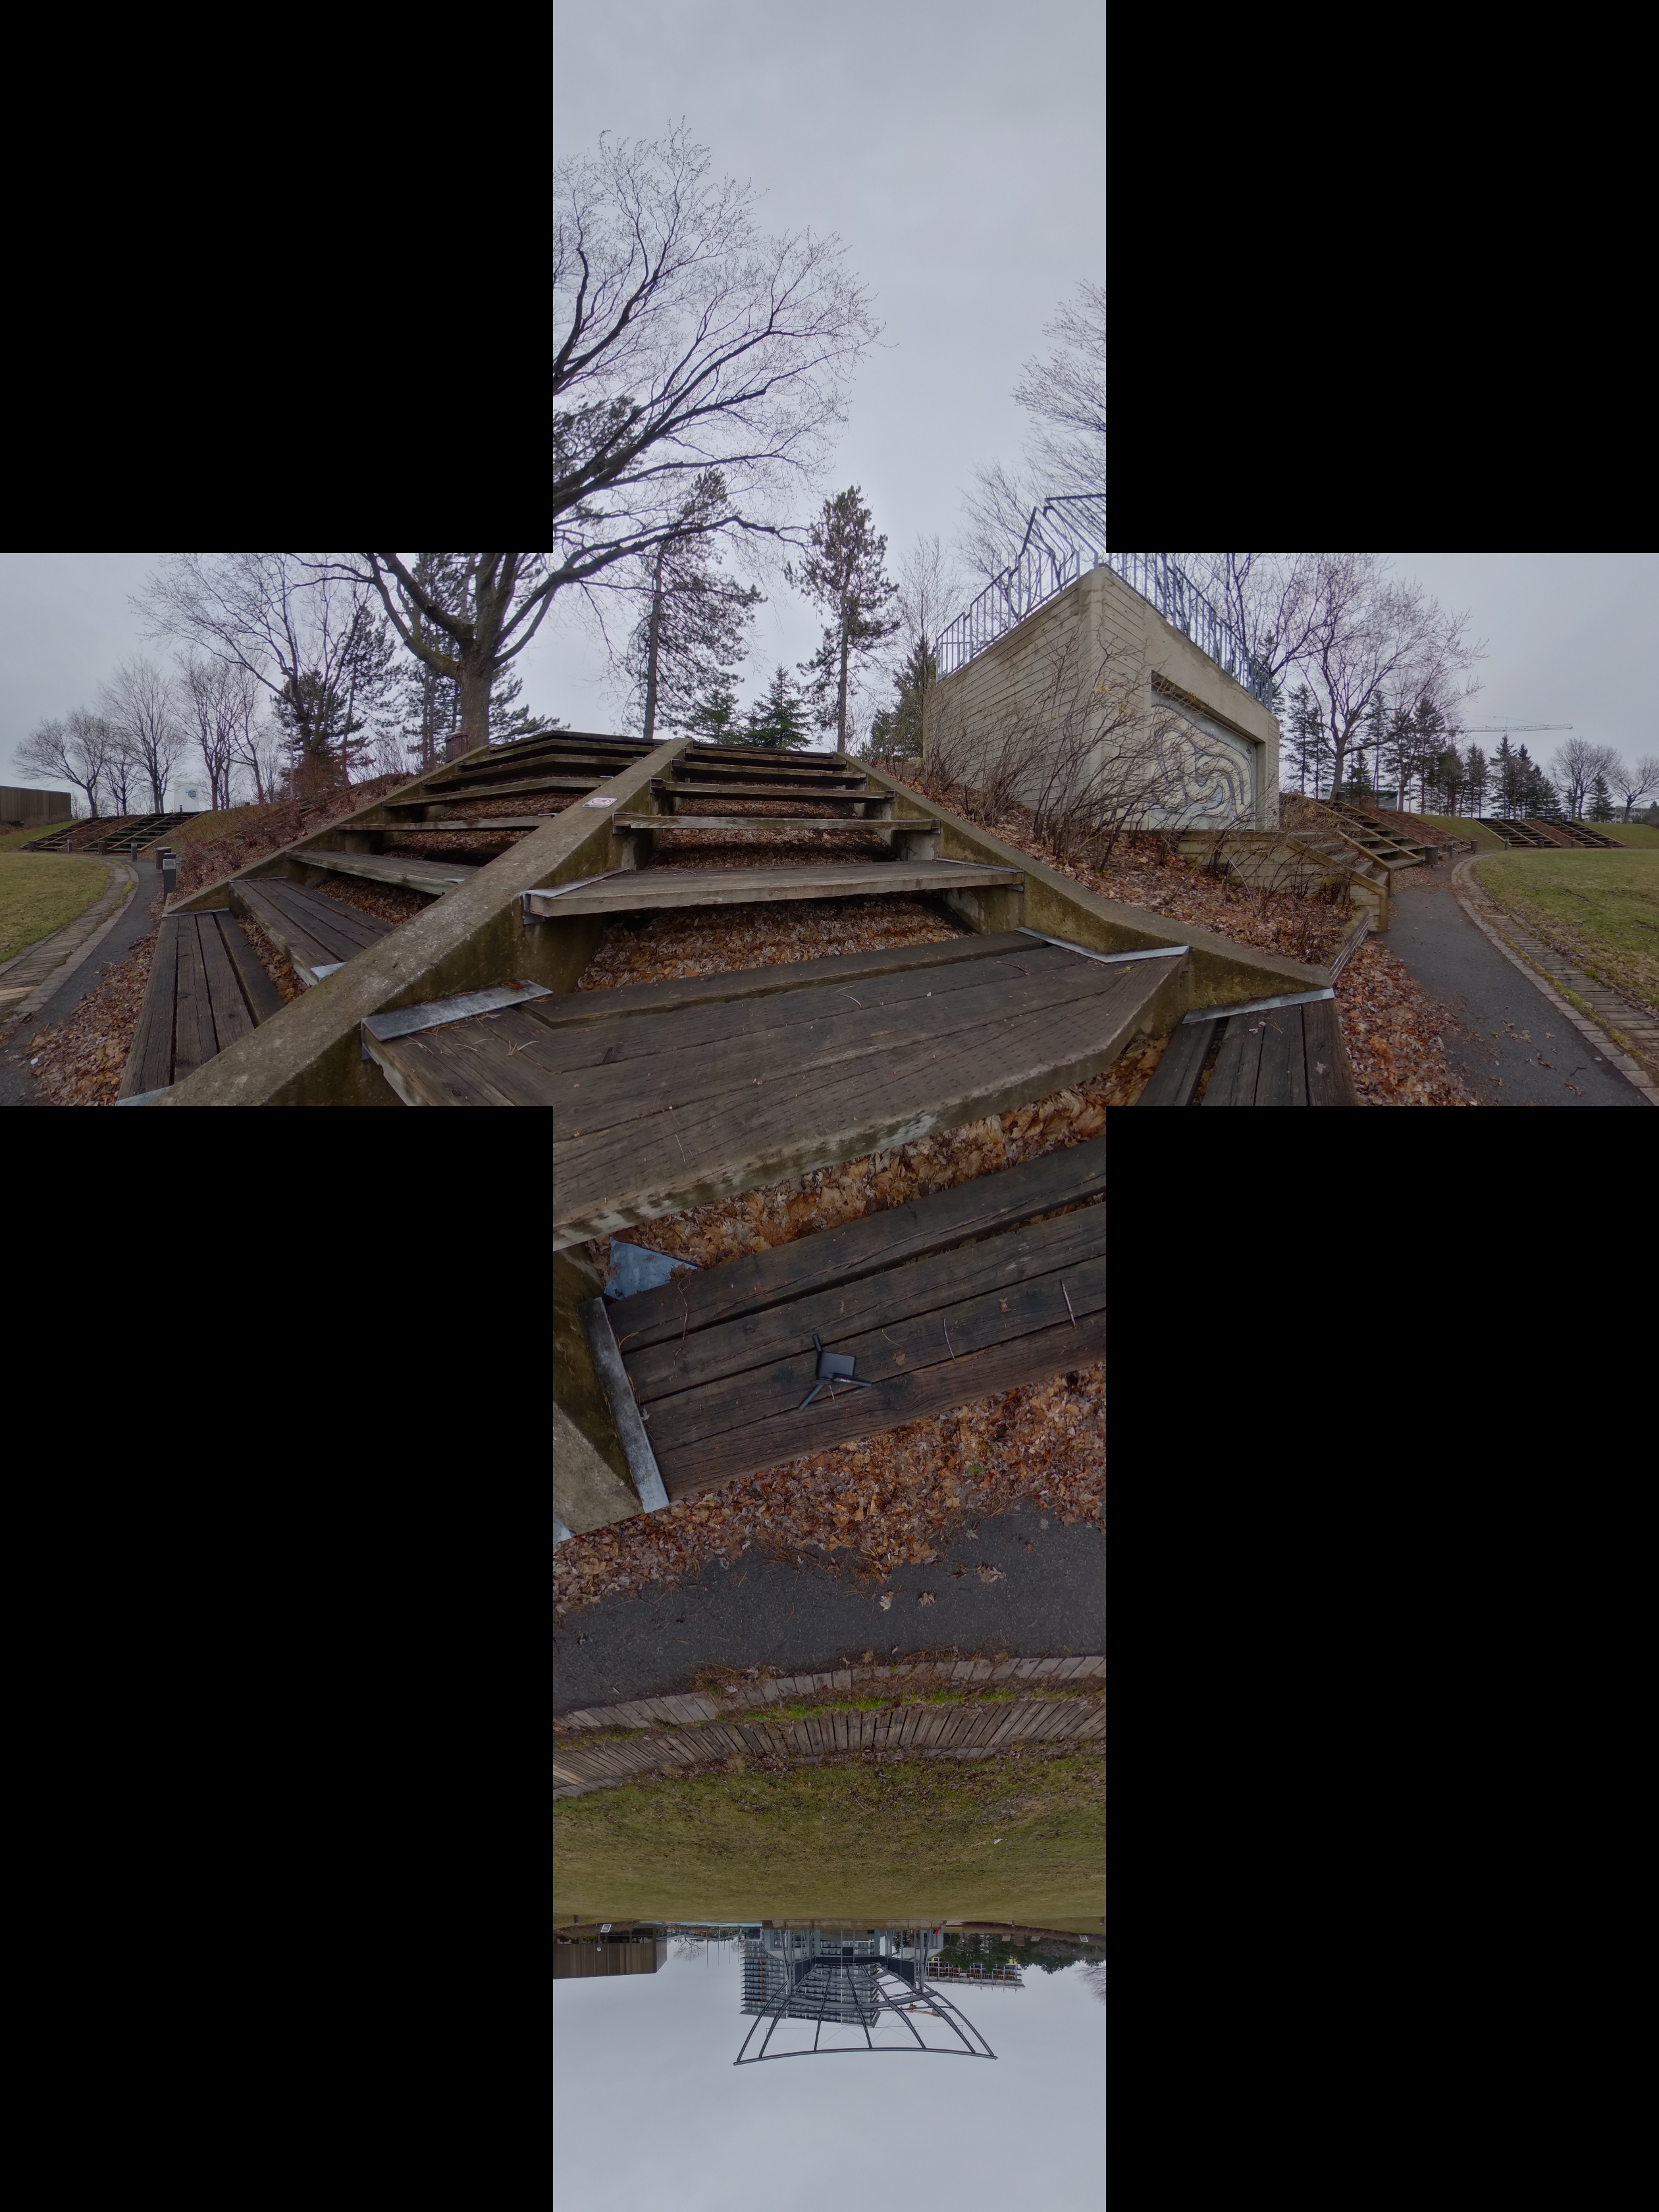
\includegraphics[width=0.5\textwidth]{02/mapping_cube_photo.jpg}
            \caption{}
%            \label{fig:SRl}
    \end{subfigure}%
     %add desired spacing between images, e. g. ~, \quad, \qquad etc.
      %(or a blank line to force the subfigure onto a new line)
    \begin{subfigure}[b]{0.5\textwidth}
            \centering
            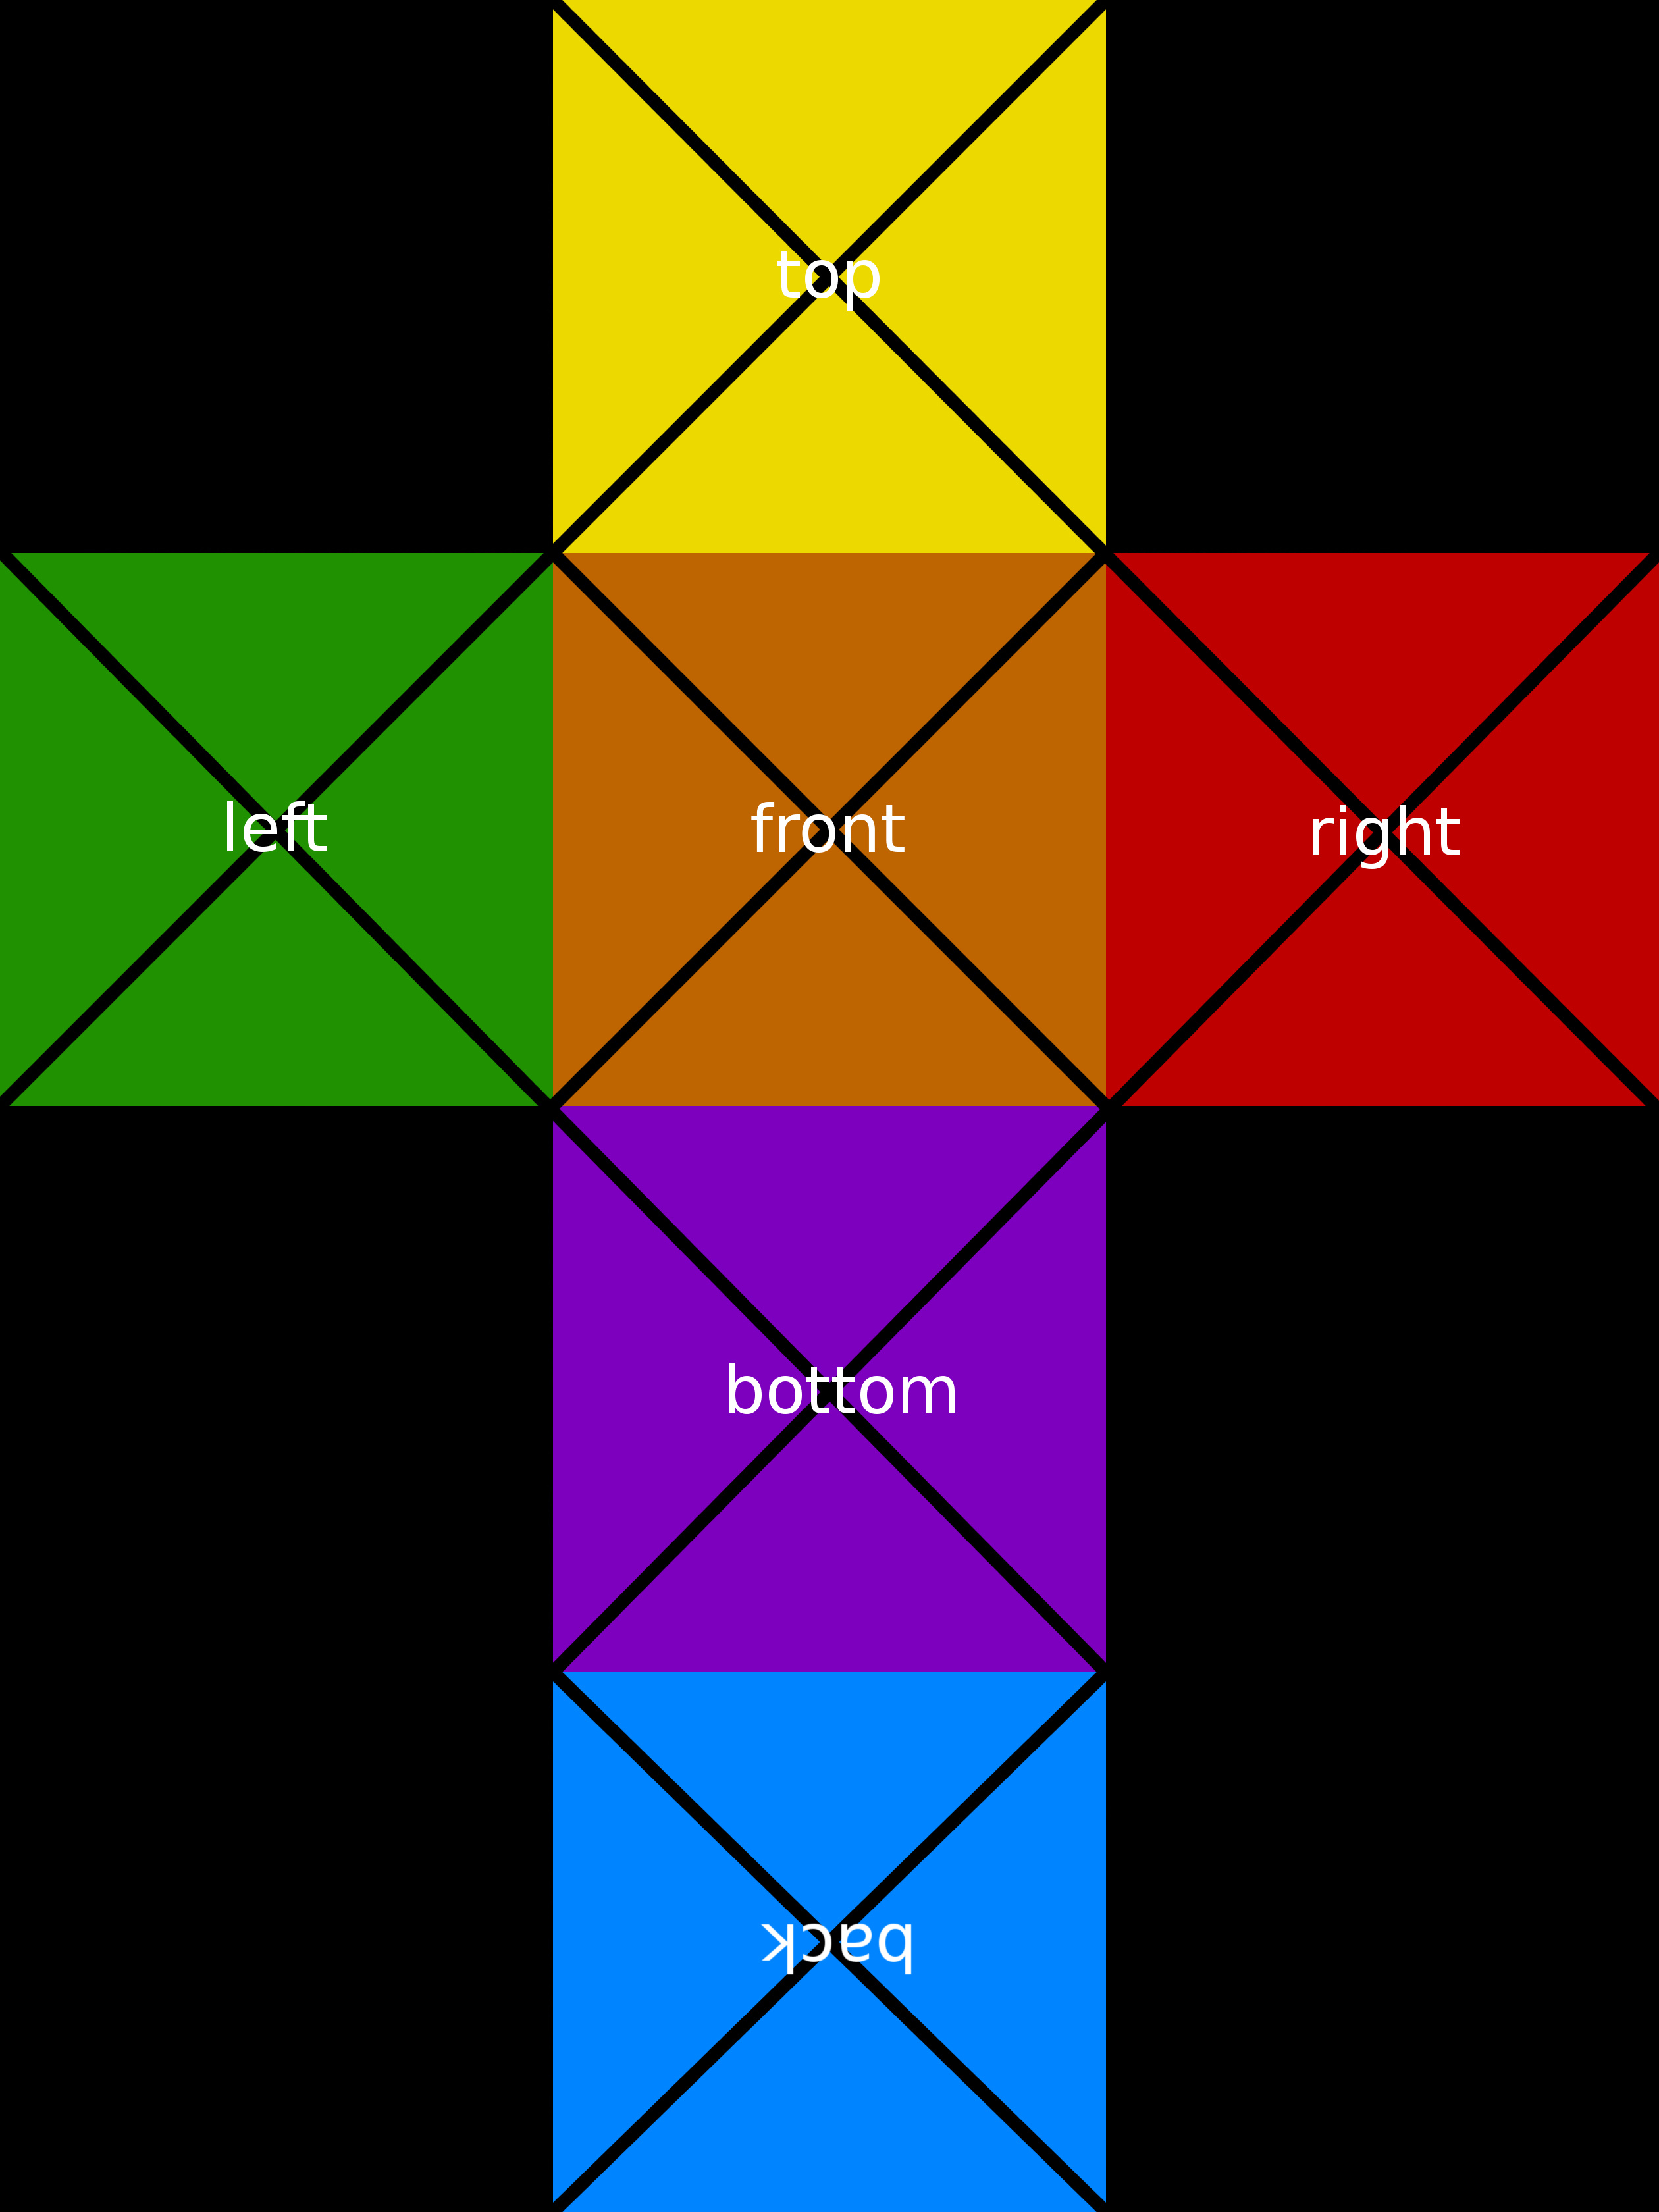
\includegraphics[width=0.5\textwidth]{02/mapping_cube.jpg}
            \caption{}
%            \label{fig:D-Imager}
    \end{subfigure}
    \caption[Cube map mapping]{The cube map mapping: (a) 360\degree image as a cube map, (b) Visualization for comparison to other mappings \protect\footnotemark}\label{fig:cubemap-intro}

    \quad
    \begin{subfigure}[b]{0.5\textwidth}            
            \centering
            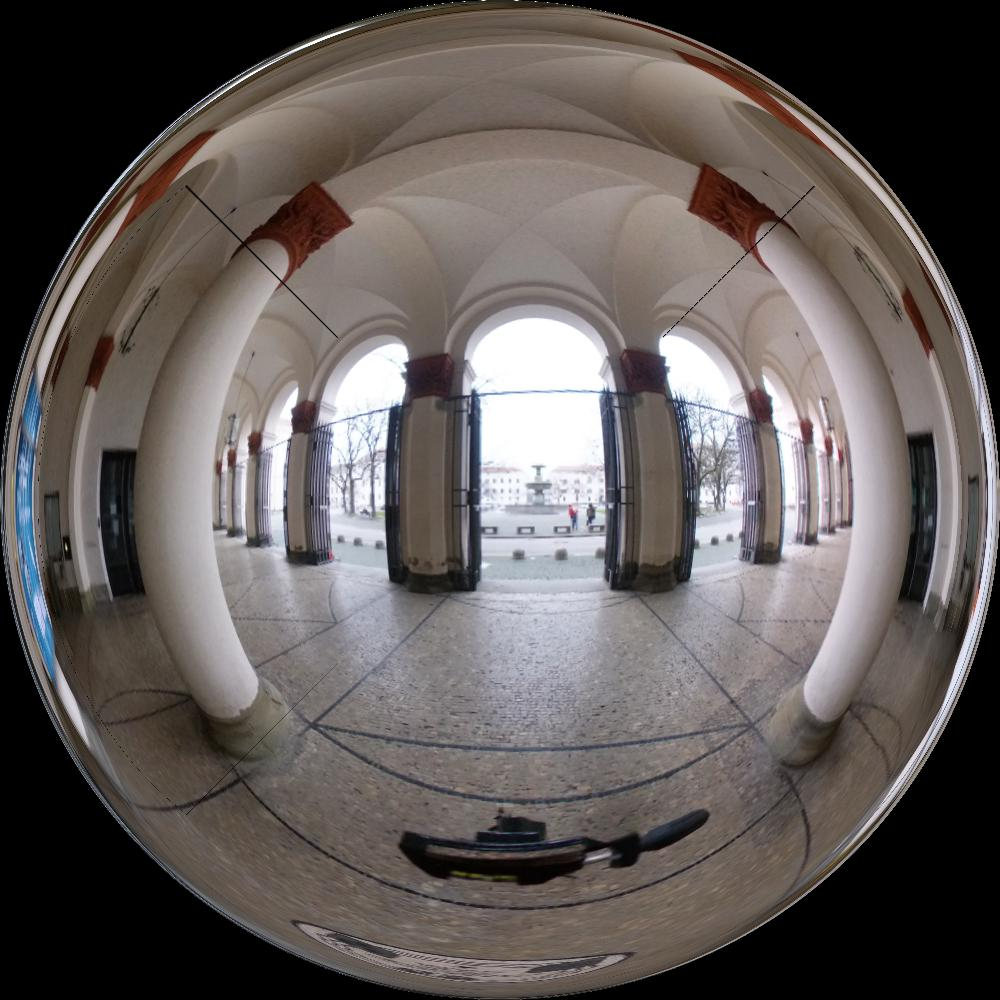
\includegraphics[width=0.5\textwidth]{02/mapping_sphere_photo.jpg}
            \caption{}
%            \label{fig:SRl}
    \end{subfigure}%
     %add desired spacing between images, e. g. ~, \quad, \qquad etc.
      %(or a blank line to force the subfigure onto a new line)
    \begin{subfigure}[b]{0.5\textwidth}
            \centering
            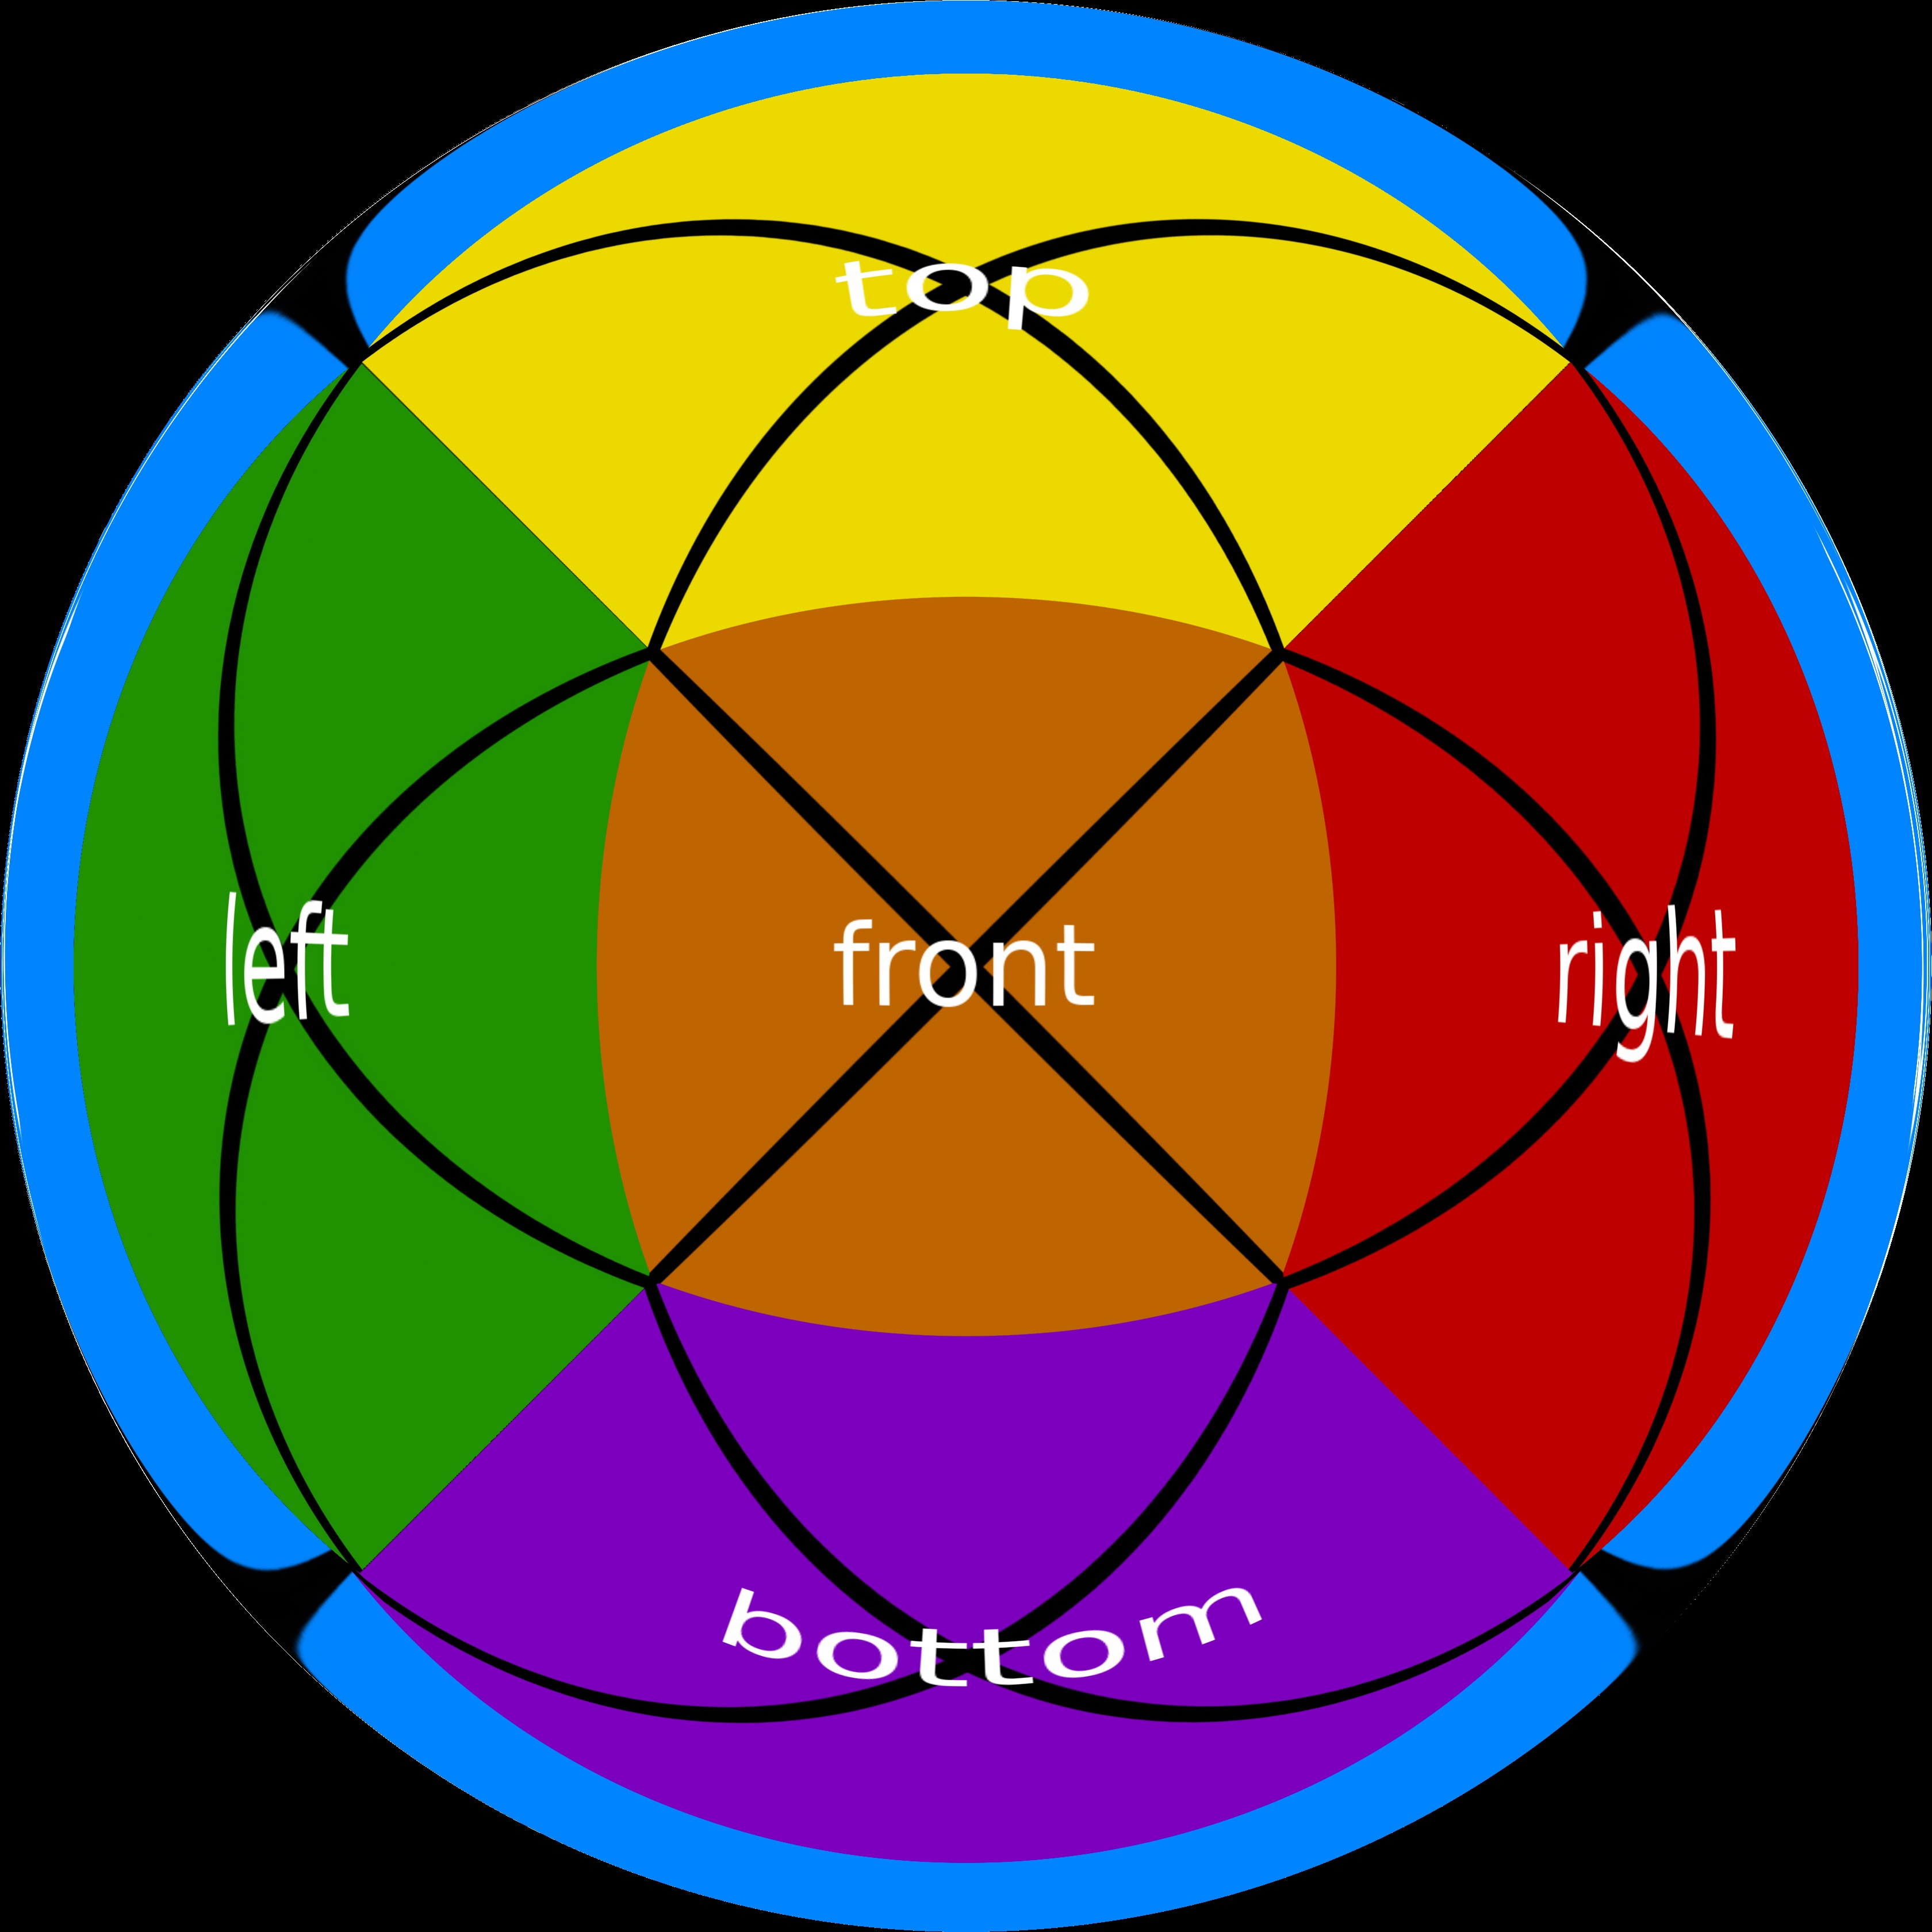
\includegraphics[width=0.5\textwidth]{02/mapping_sphere.jpg}
            \caption{}
%            \label{fig:D-Imager}
    \end{subfigure}
    \caption[Mirrored sphere mapping]{The mirrored sphere mapping: (a) 360\degree image as a mirrored sphere mapping, (b) Visualization for comparison to other mappings}\label{fig:sphere-intro}

    \quad
    \begin{subfigure}[b]{0.5\textwidth}            
            \centering
            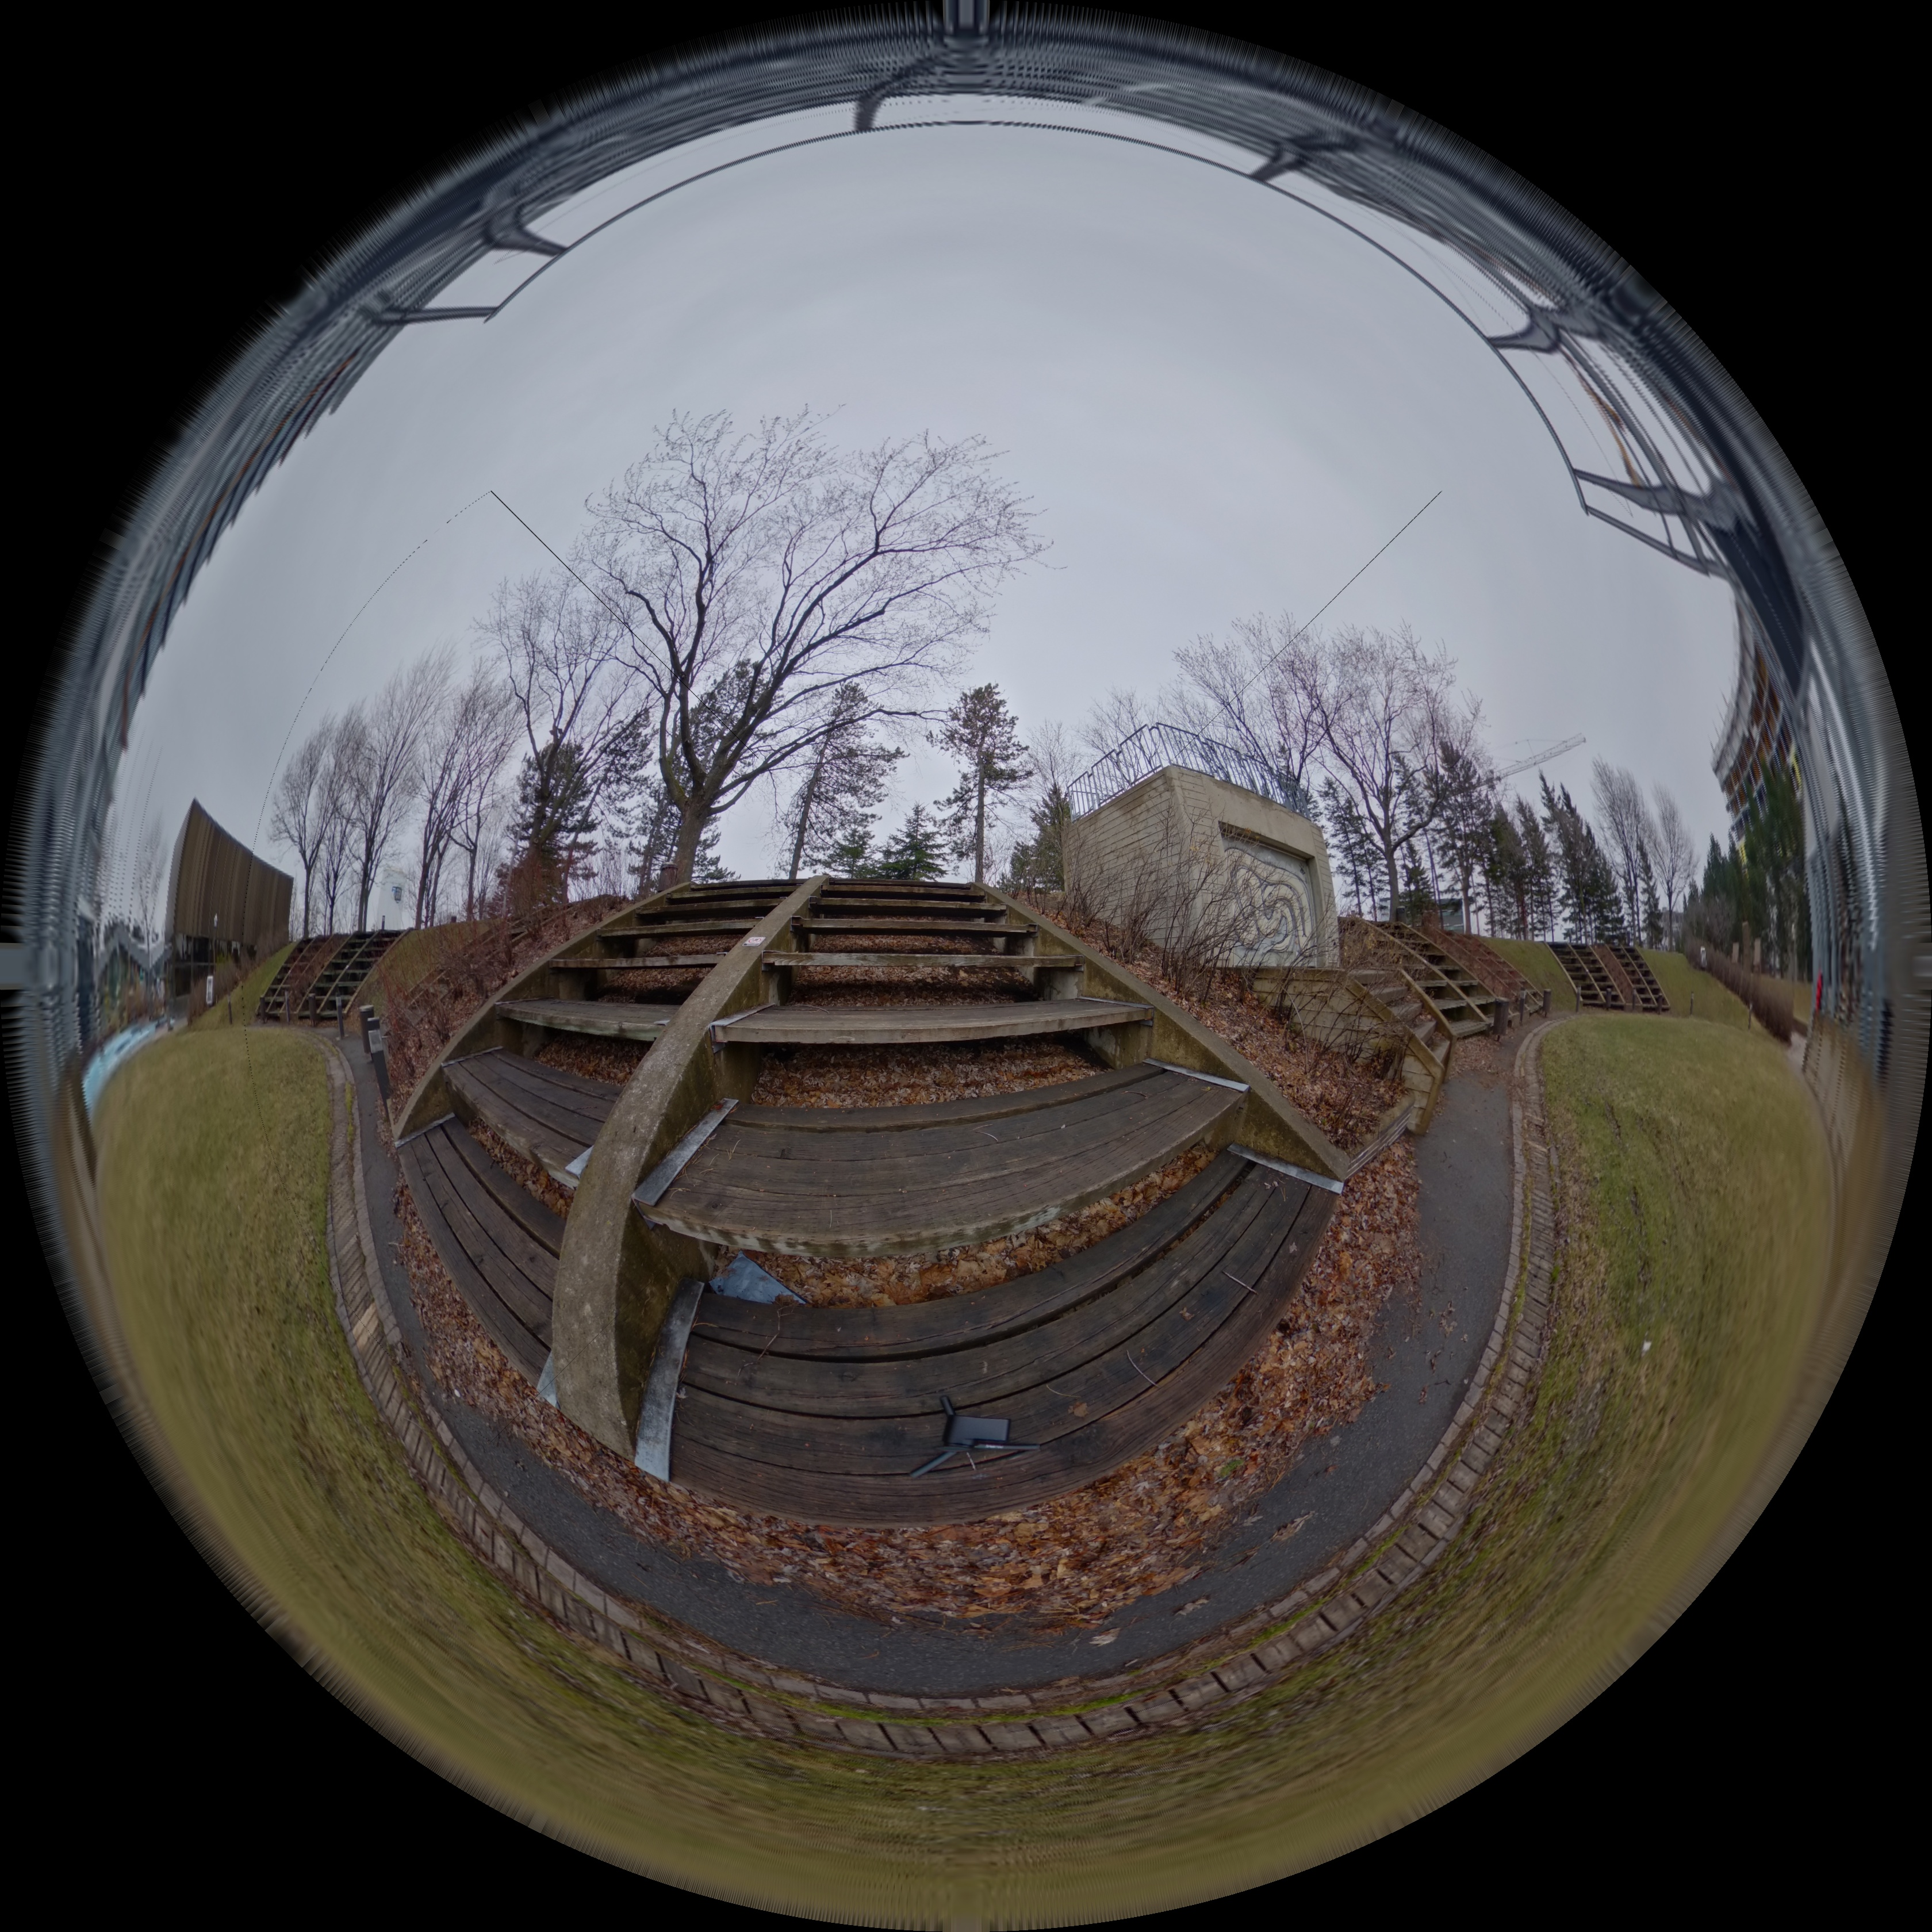
\includegraphics[width=0.5\textwidth]{02/mapping_angular_photo.jpg}
            \caption{}
%            \label{fig:SRl}
    \end{subfigure}%
     %add desired spacing between images, e. g. ~, \quad, \qquad etc.
      %(or a blank line to force the subfigure onto a new line)
    \begin{subfigure}[b]{0.5\textwidth}
            \centering
            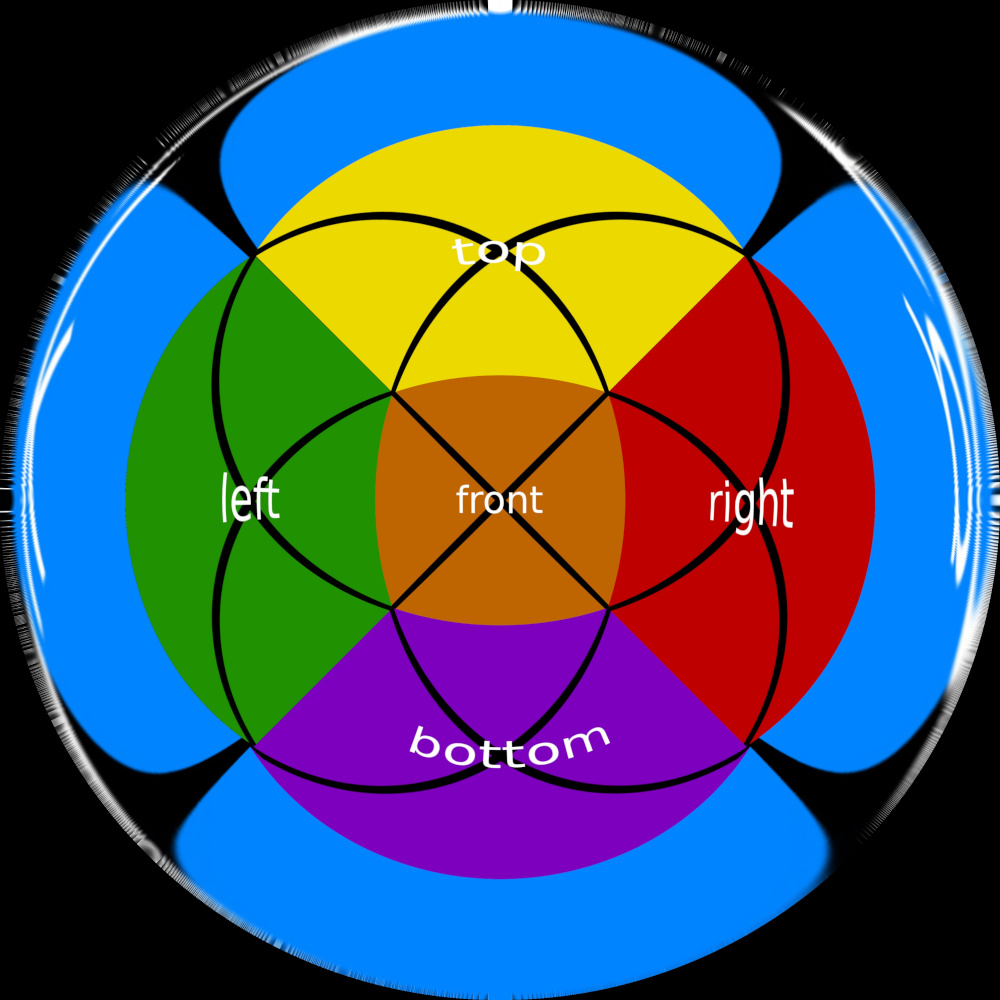
\includegraphics[width=0.5\textwidth]{02/mapping_angular.jpg}
            \caption{}
%            \label{fig:D-Imager}
    \end{subfigure}
    \caption[Angular mapping]{The angular mapping: (a) 360\degree image as an angular mapping, (b) Visualization for comparison to other mappings}\label{fig:angular-intro}

    \quad
    \begin{subfigure}[b]{0.5\textwidth}            
            \centering
            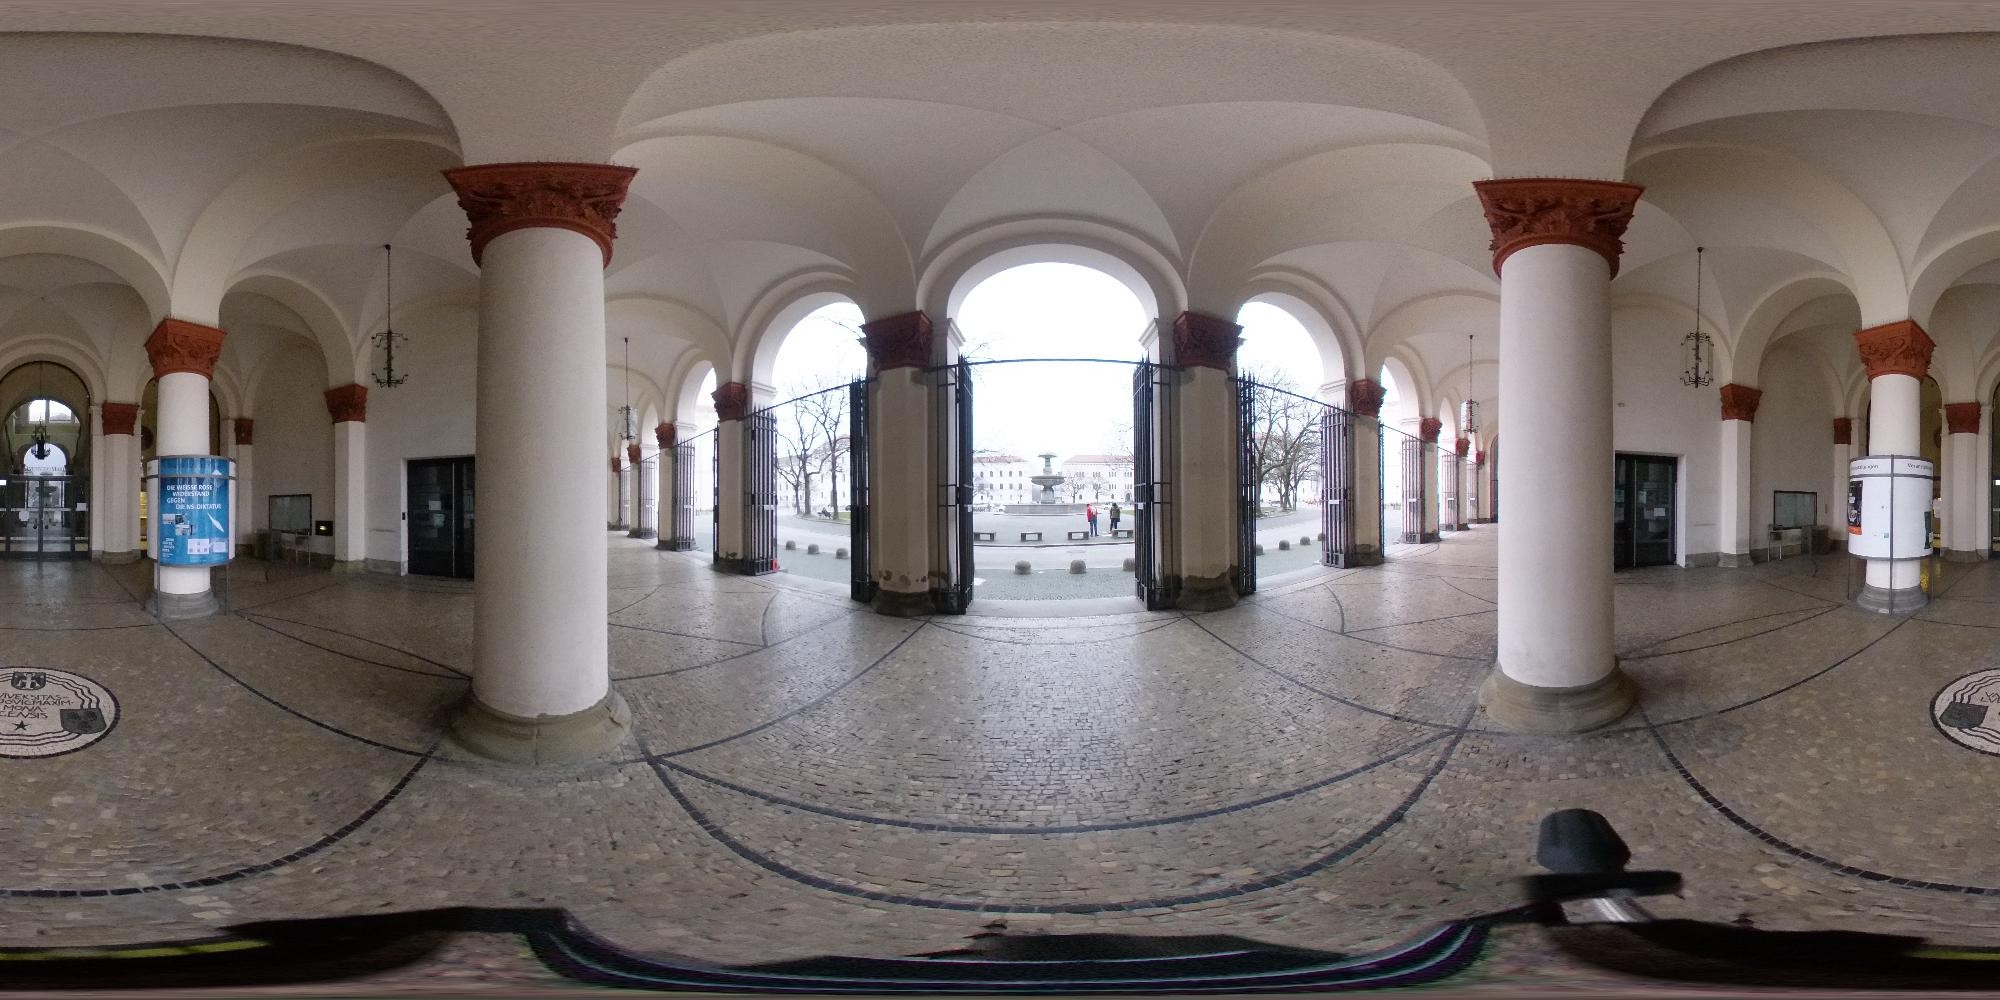
\includegraphics[width=0.9\textwidth]{02/mapping_latlong_photo.jpg}
            \caption{}
%            \label{fig:SRl}
    \end{subfigure}%
     %add desired spacing between images, e. g. ~, \quad, \qquad etc.
      %(or a blank line to force the subfigure onto a new line)
    \begin{subfigure}[b]{0.5\textwidth}
            \centering
            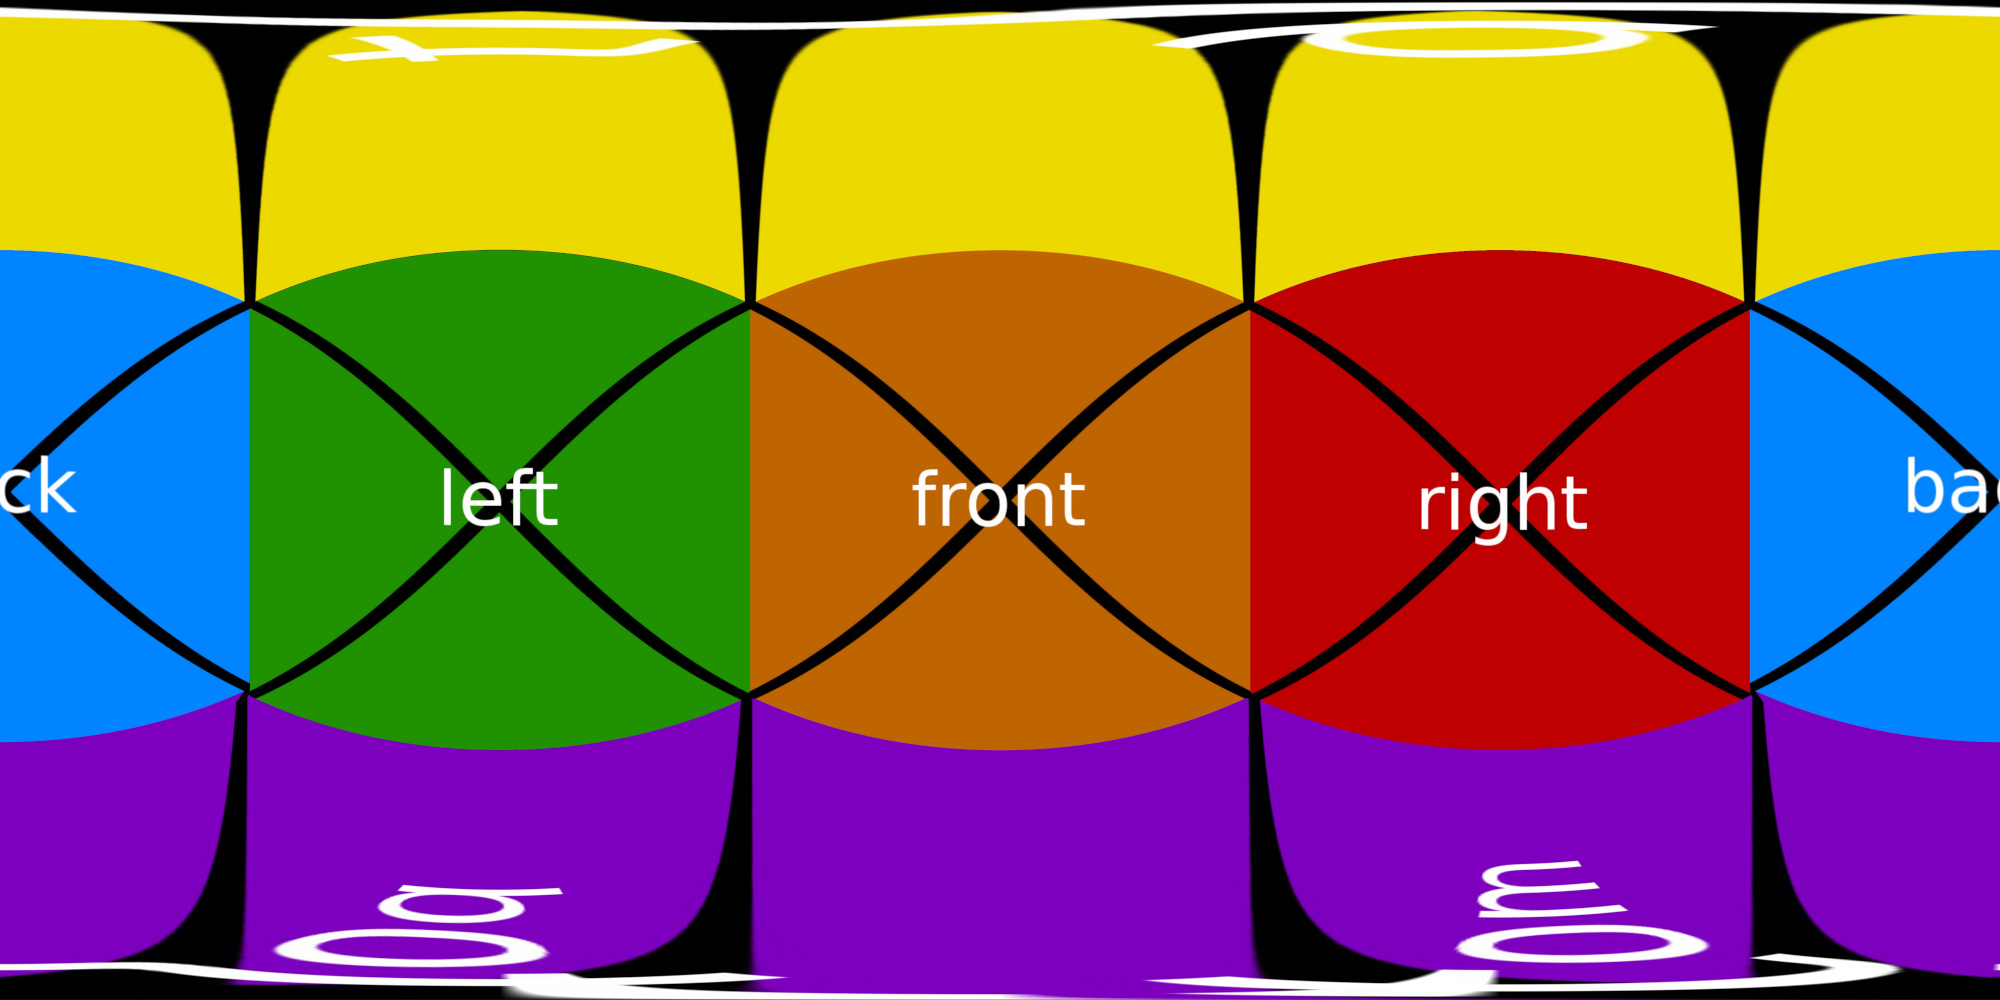
\includegraphics[width=0.9\textwidth]{02/mapping_latlong.jpg}
            \caption{}
%            \label{fig:D-Imager}
    \end{subfigure}
    \caption[Latlong mapping]{The latlong mapping: (a) 360\degree image as a latlong mapping, (b) Visualization for comparison to other mappings}\label{fig:latlong-intro}
  \end{figure}
  \footnotetext{Figure~\ref{fig:cubemap-intro}(b) does not correctly represent the distortion in cube maps. It was chosen as a baseline because cube maps have relatively small distortion compared to other mappings and it visualizes clearly which parts of the image are mapped where.}

\subsection{Optical Flow}
\subsection{Ray Tracing}

\section{Related Work}
Many approaches to image-based rendering go the path of using the 3D geometry of the scene in order to recalculate image points. The scene geometry is hereby either meticulously recorded at the time of the image capture, as with Kanade et. al's 3D Dome \cite{geometry97}, or inferred from the image data alone. Inferring 3D geometry based on planar input images has been widely examined \cite{hartley_zisserman_2004} and a number of different approaches rely heavily on this 3D geometry information, such as \ldots

Since the approach presented in this thesis is \emph{pixel-based}, i.e. using no geometry information, the following section will first outline research aiming to synthesize viewpoints with the use of little to no geometry. Then, research on image-based synthesis of 360\degree images is also examined. As the amount of research on 360\degree image synthesis is limited, approaches using geometry are also included.

\subsection{Image Synthesis without 3D Geometry for Planar Images}

\subsubsection{Megastereo \label{megastereo}}
Richardt et. al. \cite{megastereo} use a combination of image stitching and their own optical flow-based blending algorithm in order to create high resolution stereo panoramas from a set of planar images captured on a radius. The goal is to synthesize stereoscopic viewpoints (an image for the left and right eye, each) from the captured monoscopic images. After transforming the images so that they all have scene-independent orientation and minimal distortion, strips of the captured images are extracted for each ``eye'' based on the best matching image ray (Figure~\ref{fig:megastereo-figure} (a) and (b)). In cases where there is no perfect ray correspondence, the ray with the smallest deviation angle can be chosen, however, this can lead to artefacts as illustrated in Figure~\ref{fig:megastereo-figure} (c). In order to mitigate these artefacts, Richardt et. al. introduce a blending algorithm based on optical flow: 
In order to blend two images, they take the two closest viewpoints $I_K$ and $I_L$ and interpolate $\widetilde{I_M}$ using the optical flow vectors $F_{k\rightarrow l}$ and $F_{l\rightarrow k}$.  The corresponding strip is then taken from this new viewpoint which contains the matching ray (Figure~\ref{fig:megastereo-figure}~(d)).

\begin{figure}[]
\centering
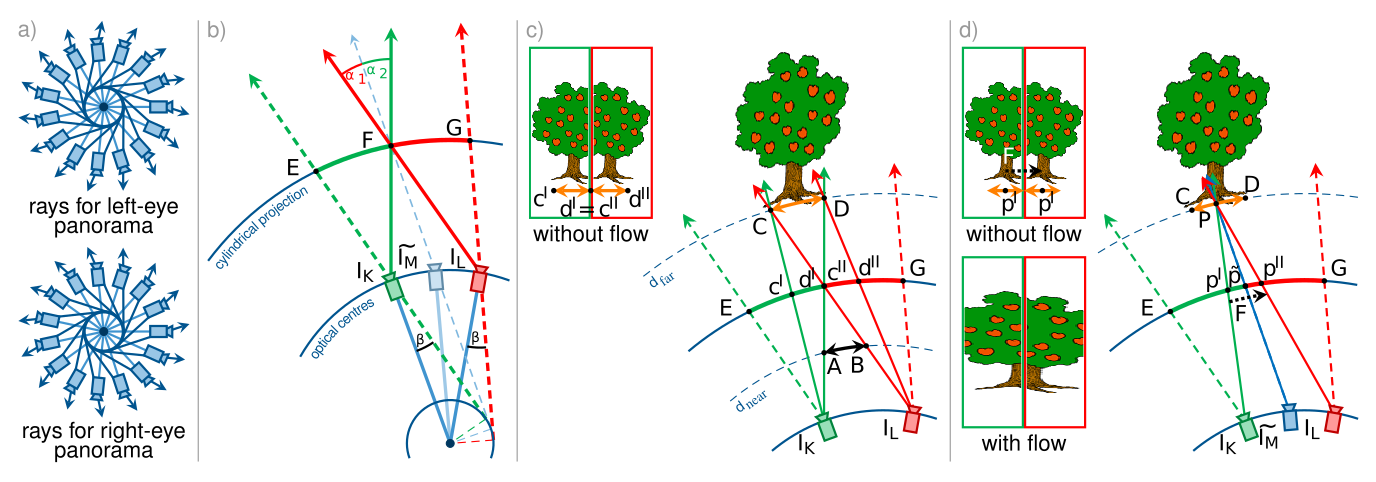
\includegraphics[width=1\textwidth]{02/megastereo-figure.png}
\caption[Flow-based blending in Megastereo]{(a) Illustration of rays required for creating a stereoscopic panorama and (b) deviation angle $\beta$. (c) Duplication and truncation artefacts caused by the aliasing. (d) Flow-based upsampling to synthesize required rays. \emph{From \cite{megastereo}}}
\label{fig:megastereo-figure}
\end{figure}

For Megastereo, there is no need to blend the complete images, instead, they restrict their calculations to the strips/pixels they need. For simplicity's sake, the process is described for a full image:
The interpolated image $\widetilde{I_M}$ at point $\alpha$ between the images $I_K$ and $I_L$ is calculated by shifting $I_K$ by $\alpha \cdot F_{k\rightarrow l}$ and by shifting $I_L$ by $(1 - \alpha) \cdot F_{l\rightarrow k}$. The two shifted images are then blended linearly, using $\alpha$ as the weight.

\begin{itemize}
  \item other approaches, such as light field approaches or neural network approaches
\end{itemize}

\subsection{Image Synthesis for 360\degree Images}

\subsubsection{6-DOF VR Videos with a Single 360-Camera}
Huang et. al. \cite{6dof} propose a method to expand regular 360\degree video data into stereoscopic video data viewable with six degrees of freedom. Their approach is based on reconstructing the 3D scene and the camera path. This reconstruction is achieved by adapting well-established structure-from-motion (SfM) algorithms for 360\degree data. Since SfM algorithms are designed for planar images with a limited field of view (FoV), the six separate faces of the cube map representation are used as input for the SfM algorithm. SfM algorithms work by tracking points across a series of images (e.g. frames), so for cube mappings, potential points moving across seams need to be accounted for. This is done by extending the field of view of each face so that regions around seams are represented on both sides of the seam. After the points are correctly tracked, the extended cube map is reduced back to its original format. Then, the sparse scene geometry and camera path are calculated by incrementation and interpolation. The sparse geometry is then refined to a dense reconstruction of the scene using depth maps and Delaunay Triangulation. Finally, new viewpoints are synthesized by warping the current frame. Their warping algorithm projects the dense 3D points to a unit sphere control mesh with icosahedral tesselation\footnote{Icosahedral tesselation of a sphere subdivides the surface of a sphere into triangles. Other terms for this type of sphere are Icosphere or Geodesic Polyhedron} for both the captured viewpoint and the desired viewpoint. Then the vertex motion between each pair of triangles is calculated and the image warped according to these motion vectors (see Figure~\ref{6dof-figure}). 

\begin{figure}[]
\centering
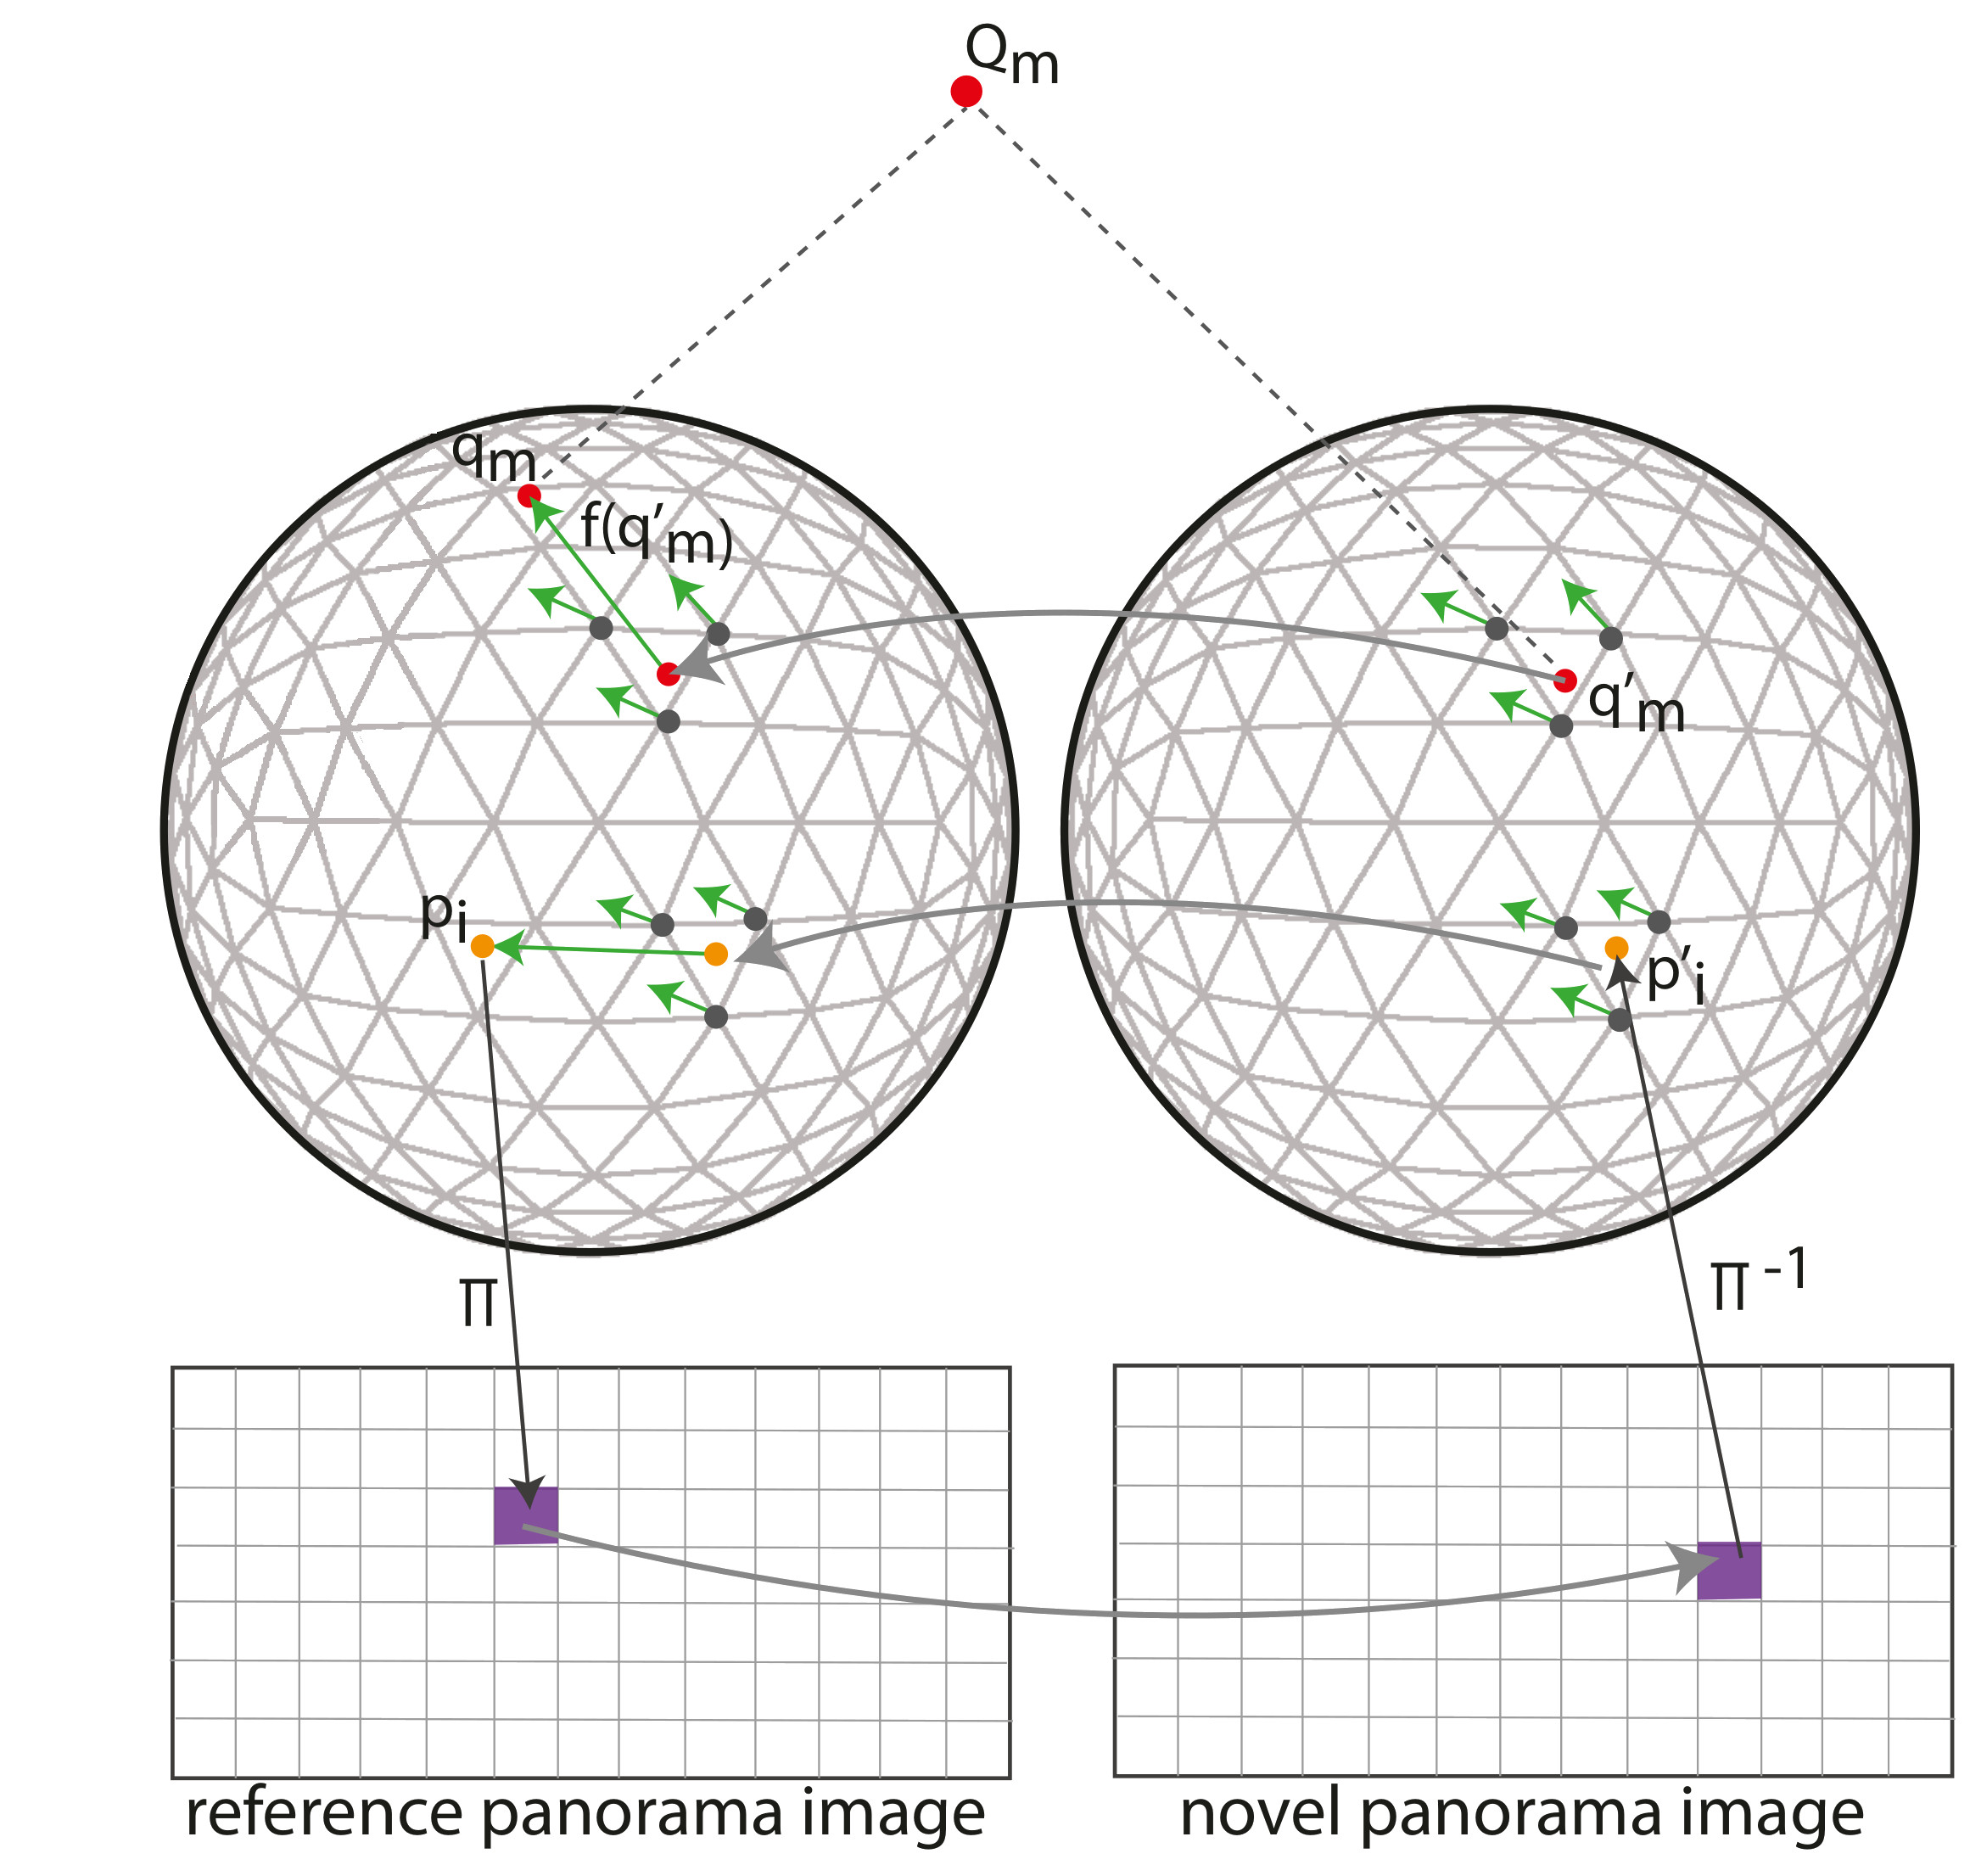
\includegraphics[width=0.6\textwidth]{02/6dof-figure.jpg}
\caption[Image warping from Huang et. al.]{. \emph{adapted from \cite{6dof}}}
\label{fig:megastereo-figure}
\end{figure}

\subsubsection{Panorama Image Interpolation for Real-time Walkthrough}
\cite{walkthrough}

\subsubsection{On the Use of Ray-tracing for Viewpoint Interpolation in Panoramic Imagery}
\cite{raytracing}

